% Clean reading-layout version of the paper manuscript.
% The substantive drafting source remains paper.md; this file exists so the
% repo can generate a more polished PDF than a browser-print export.
\documentclass[11pt,letterpaper]{article}

\usepackage[utf8]{inputenc}
\usepackage[T1]{fontenc}
\usepackage[margin=1in]{geometry}
\usepackage{graphicx}
\usepackage{amsmath}
\usepackage{booktabs}
\usepackage{array}
\usepackage{tabularx}
\usepackage{abstract}
\usepackage{caption}
\usepackage[hidelinks]{hyperref}
\usepackage{xurl}
\usepackage{setspace}
\usepackage{titlesec}

\graphicspath{{build/figures/}{../figures/}}

\setlength{\parindent}{0pt}
\setlength{\parskip}{0.65em}
\setlength{\emergencystretch}{2em}
\setlength{\textfloatsep}{14pt plus 2pt minus 3pt}
\setlength{\floatsep}{12pt plus 2pt minus 2pt}
\setlength{\intextsep}{12pt plus 2pt minus 2pt}
\setlength{\absleftindent}{1.2em}
\setlength{\absrightindent}{1.2em}
\setlength{\absparsep}{0.5em}
\captionsetup{font=small, labelfont=bf, justification=raggedright, singlelinecheck=false, skip=8pt}
\titlespacing*{\section}{0pt}{1.35\baselineskip}{0.55\baselineskip}
\titlespacing*{\subsection}{0pt}{1.1\baselineskip}{0.45\baselineskip}

\newcolumntype{L}[1]{>{\raggedright\arraybackslash}p{#1}}
\newcolumntype{C}[1]{>{\centering\arraybackslash}p{#1}}
\newcolumntype{R}[1]{>{\raggedleft\arraybackslash}p{#1}}

\begin{document}

\begin{center}
{\LARGE\bfseries Selective Entry and Structured Electricity-Recovery Performance in Japan's Waste-Incineration Fleet: A Facility-Level Panel Study\par}
\vspace{1.05em}
{\large Pann Phetra\par}
\vspace{0.2em}
\small
College of Sustainability and Tourism, Ritsumeikan Asia Pacific University, 1-1 Jumonjibaru, Beppu, Oita 874-8577, Japan\par
\vspace{0.45em}
Corresponding author: \href{mailto:ph23p2dl@apu.ac.jp}{ph23p2dl@apu.ac.jp}\par
\end{center}
\normalsize
\vspace{0.45em}

\begin{abstract}
Japan relies heavily on municipal waste incineration, yet by fiscal year (FY) 2024 only 41.1\% of facilities in the panel are flagged as power-generating. Fleet-average studies blur the entry of facilities into electricity recovery with performance among existing generators. Using Ministry of the Environment data for FY2005--FY2024, this paper estimates both margins in one national facility panel. The entry event is first observed reporting of positive installed generation capacity. Facilities older than ten years are less likely to record this event in the next fiscal year, while larger facilities are more likely to do so. The definition maps closely to operation: 135 of 141 entrants report positive electricity output by the following year. A separate diagnostic shows that older non-entrants are more likely to disappear from the coded panel, although panel exit is not verified closure. Among identifiable operating generators, bounded gross electricity generation per tonne is lower at older plants and higher at larger, more fully utilized plants. Between-facility heterogeneity dominates within-facility movement, and adjacent-year performance ranks correlate at 0.93. These linked patterns are descriptive, not causal estimates of one modernization mechanism. They show that installed-capacity entry, administrative attrition, and generator performance are distinct observed outcomes. Municipal fleet planning should therefore not manage facilities outside electricity recovery and mature generators as one average segment.
\end{abstract}

\vspace{0.2em}
\noindent\textbf{Keywords:} waste incineration; waste-to-energy; Japan; energy recovery; facility panel; transition
\vspace{0.35em}

\section{Introduction}

Japan operates one of the world's most incineration-dependent municipal waste systems, yet many facilities still burn waste without generating electricity from the heat they produce (Ministry of the Environment Japan, 2026; Uno, 2015; Tabata \& Tsai, 2016; Sakai et al., 2011). In fiscal year (FY) 2024, 41.1\% of facilities in the panel are flagged as power-generating, leaving most facilities outside electricity recovery. This is not a marginal technical detail. For decades, Japanese municipal waste governance has relied on thermal treatment for hygienic disposal, volume reduction, and local waste autonomy, while limited landfill space and strict environmental controls pushed municipalities toward sophisticated incineration infrastructure (Brunner \& Rechberger, 2015; Sakai et al., 2011). Sectoral planning now treats the remaining electricity-generation gap as part of the waste sector's decarbonization challenge (Yamada et al., 2023; Greenhouse Gas Inventory Office of Japan \& Ministry of the Environment Japan, 2024). The transition problem is therefore not whether Japan uses incineration. It is whether observed entry into electricity recovery is patterned across facilities and how electricity recovery intensity varies once generation is present.

Aggregate fleet summaries flatten two distinct questions. One is extensive: which facilities first report installed power-generation capacity? The other is intensive: among plants that already generate, which facilities achieve high electricity recovery per tonne? The system can therefore look uniformly slow in the mean while combining selective entry at one end of the fleet with persistent performance hierarchy at the other.

\subsection*{Research questions}

This paper asks two descriptive empirical questions and one interpretive synthesis question. In the list, RQ denotes research question; the synthesis item states how the two empirical results are read together:

\begin{description}
\item[RQ1: Entry margin.] Among coded facilities first observed without installed power-generation capacity, which prior-year age and capacity profiles are associated with first observed reporting of positive installed generation capacity in the following fiscal year?
\item[RQ2: Generator-performance margin.] Among identifiable operating generators, how is electricity recovered per tonne associated with facility age, design capacity, utilization, heating value, and common fiscal-year conditions?
\item[Synthesis.] Taken together, do the observed entry pattern and generator-frame performance associations support one average-fleet modernization interpretation, or do they indicate distinct adoption and performance problems within the same incineration system?
\end{description}

The contribution is not a causal estimate of retrofit effects or a technical optimization model. It is a linked facility-panel decomposition that shows why observed entry into generation and conditional generator performance should be modeled separately before being interpreted together. The paper uses two linked samples: one follows non-generating facilities until they first report electricity generation, and the other compares identifiable operating generators over time. In the first sample, observed transition is selective toward younger and larger facilities. In the second, electricity recovery intensity is strongly structured by age, scale, and utilization, while within-facility movement remains limited relative to between-facility heterogeneity. The same fleet can therefore look merely slow in aggregate while containing two different problems: selective entry into generation and persistent generator hierarchy. For municipal planning, that distinction changes the first diagnostic step. Facilities outside electricity recovery and mature generators should be evaluated as different asset-management questions before they are summarized as one fleet.

A natural expectation is that younger and larger plants will have advantages. The contribution is not that age and scale matter in isolation. It is that the same administrative fleet shows those advantages on two different margins: younger and larger facilities are overrepresented in observed entry into generation, while operating generators remain stratified after entry. That two-margin structure is what an aggregate fleet mean or generator-only study would miss. It turns a familiar expectation into a sharper diagnostic: the question is not only whether newer and larger plants perform better, but whether the fleet's entry problem and post-entry performance problem are actually the same problem.

\begin{figure}[t]
\centering
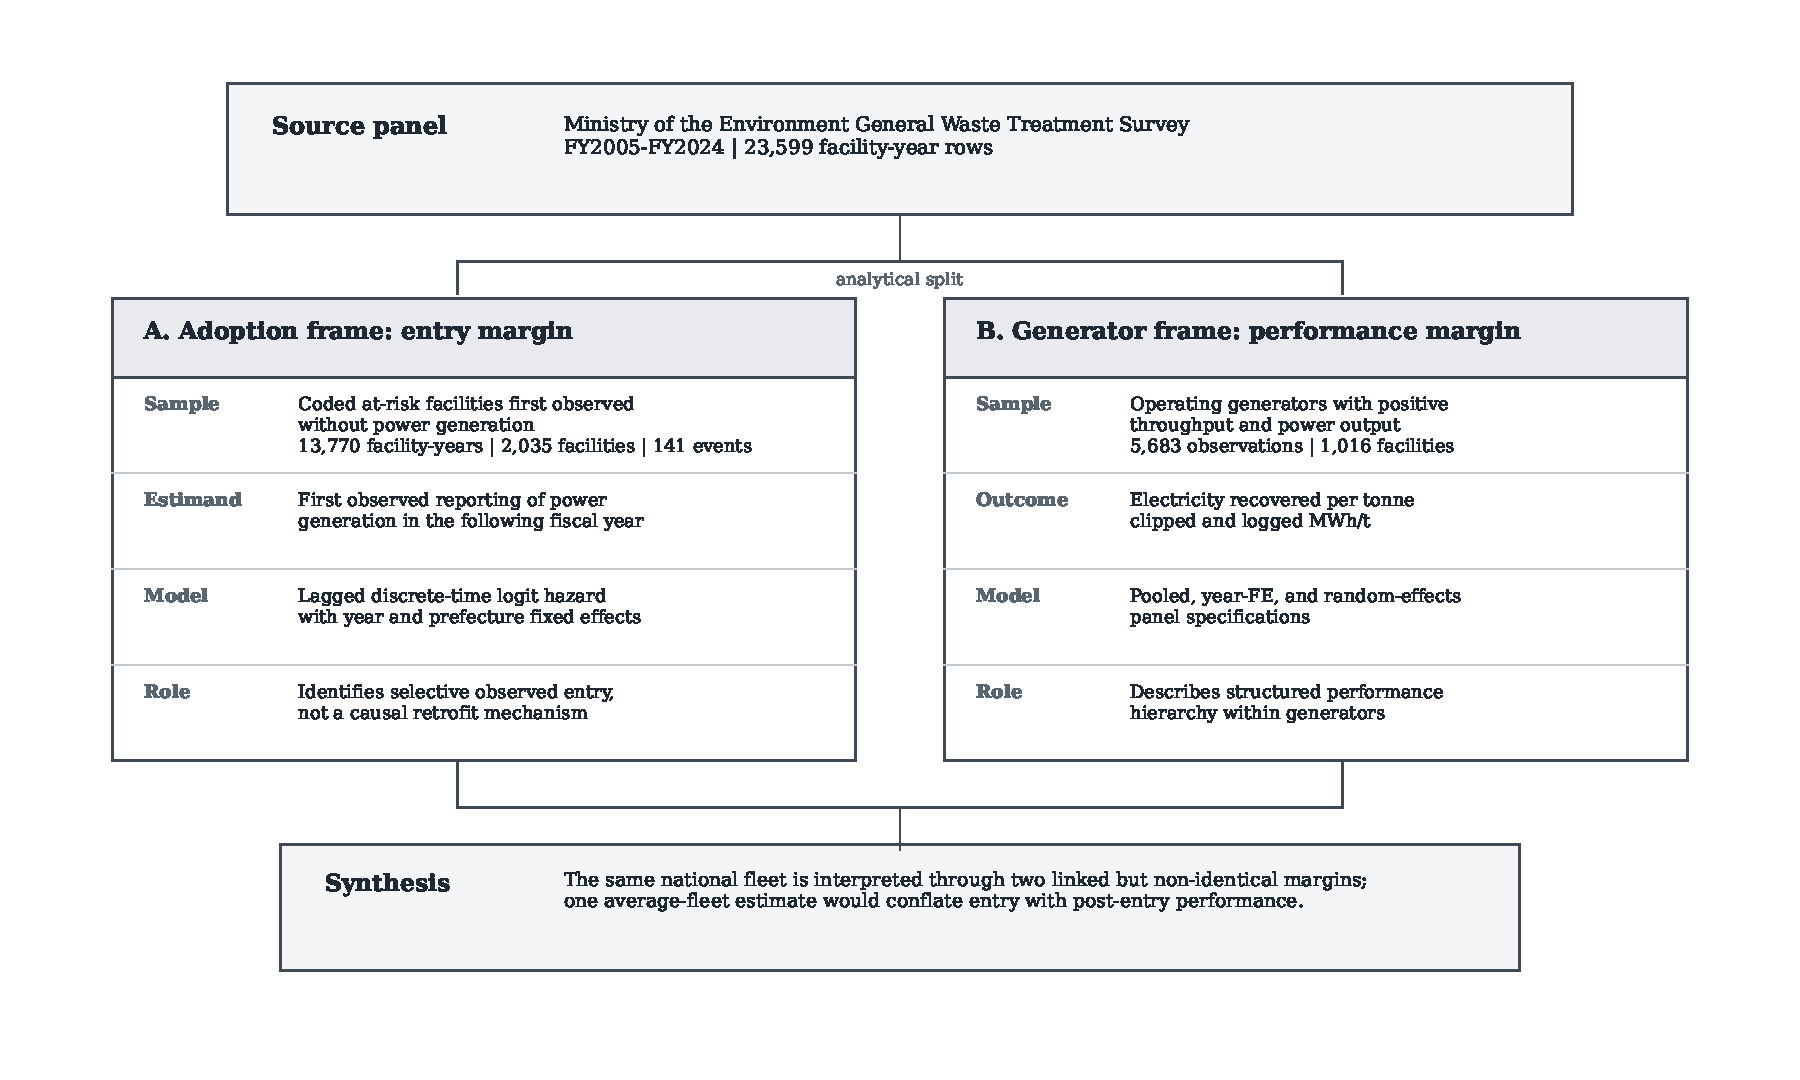
\includegraphics[width=0.98\textwidth]{figure1_two_part_framework.pdf}
\caption{Analytical design separating the source panel into entry and generator-performance margins before interpreting both margins together.}
\end{figure}

The gap addressed here is narrower than a generic claim that Japan has been understudied. Waste-to-energy research can describe fleet trajectories, and generator-only studies can explain conditional performance once plants already operate as generators. What remains uncommon is one linked municipal-fleet analysis that estimates both margins and asks whether they point to the same modernization bottleneck. Japan makes that contrast visible because persistent non-generators, old small plants, and a more modern generating segment coexist in the same administrative system. In such mixed fleets, adoption and conditional performance should be modeled separately before they are interpreted together.

The rest of the paper proceeds as follows. Section 2 positions the paper against the literature most relevant to the analytical split. Section 3 introduces the two linked analytical frames and the main estimation choices. Section 4 reports the adoption and electricity-recovery results in sequence, then ties them together. Section 5 interprets the combined finding, explains what the data still cannot identify, and states a short set of evidence-consistent implications. Section 6 concludes.

\section{Literature Positioning}

This paper speaks to three literatures that often meet in practice but start from different empirical positions: waste-to-energy systems, facility-level performance analysis, and infrastructure lock-in. The review is organized around the paper's central split between entry into generation and conditional performance after entry. The relevant gap is not simply that Japan needs another case study. It is that existing studies often describe fleets in aggregate or explain generator performance conditional on operation, yet rarely estimate both margins in one linked municipal-fleet design.

Work on waste-to-energy systems often documents national trajectories, technology choices, or lifecycle implications of thermal treatment (Astrup et al., 2009; Astrup et al., 2015; Brunner \& Rechberger, 2015; Sun et al., 2018). Japan-specific work has mostly emphasized technology upgrading, heat-use constraints, and sectoral decarbonization scenarios rather than facility-level transition modeling (Uno, 2015; Tabata \& Tsai, 2016; Yamada et al., 2023). Policy-facing work reaches a similar conclusion from a different angle: waste-to-energy is treated as useful only when embedded in a wider waste hierarchy and resource-recovery strategy rather than as a stand-alone justification for thermal treatment (European Commission, 2017; Sakai et al., 2011). This literature is indispensable for understanding why energy recovery matters, but it usually treats the incineration fleet as a sectoral category. It can show whether energy recovery is expanding, whether heat supply remains constrained, or whether the sector matters for net-zero planning. It is less well suited to distinguishing facilities that enter generation from those that do not.

Facility-level performance studies are closer to the present design, but they typically begin after entry has already occurred. Studies in Taiwan, for example, evaluate operating incinerators by decomposing waste-treatment, electricity-generation, or revenue performance within existing plants (Chen et al., 2012; Yeh, 2020). Other work focuses on energy-recovery criteria, plant scale, heat use, and the system consequences of different waste-to-energy configurations (Grosso et al., 2010; M\"{u}nster \& Meibom, 2010). Recent Chinese plant-level work is also highly informative about performance differentials inside the generating segment and the effectiveness of upgrading strategies at scale (Cui et al., 2026; Liu et al., 2025; Han et al., 2025). Those studies help define the intensive-margin question. They do not directly answer which non-generating facilities enter generation in the first place.

The present paper therefore uses those comparator papers as a method-positioning map rather than as templates to copy. The map below makes the adaptation logic explicit.

\begin{center}
\scriptsize
\renewcommand{\arraystretch}{1.15}
\textbf{Comparator adaptation of research logic}\\[0.45em]
\begin{tabularx}{\textwidth}{L{2.55cm} X X X}
\toprule
Source family & Borrowed logic & Japan-specific adaptation & Not claimed here \\
\midrule
Cui et al. (2026) & Incinerators form a performance hierarchy, not interchangeable plants & The Japan panel is read through facility heterogeneity and persistent hierarchy & No optimization frontier or ranking of Japanese plants on the same technical frontier \\
Liu et al. (2025) & Waste-energy systems should be judged by effectiveness, not expansion alone & Effectiveness is split into entry into generation and performance after entry & No China-style waste-energy-carbon development model \\
Han et al. (2025) & Resource recovery and sustainability depend on upgrade pathways, not incineration alone & Resource-recovery framing is kept while using variables available in the Japanese administrative panel & No pollutant-control technology model because comparable plant-level variables are unavailable \\
Chen et al. (2012) and Yeh (2020) & Facility-level incinerator performance can be compared after operation begins & The generator frame models electricity recovered per tonne across identifiable plants & No data envelopment analysis frontier or electricity-revenue inefficiency model \\
Grosso et al. (2010) and M\"{u}nster and Meibom (2010) & Energy recovery should be interpreted in a wider energy-system context & Gross electricity generation per tonne provides an applied recovery measure & No full R1 efficiency calculation, net-export measure, lifecycle balance, or energy-system optimization model \\
\bottomrule
\end{tabularx}
\renewcommand{\arraystretch}{1}
\normalsize
\end{center}

This matters for interpretation because the paper is not trying to be a weaker version of any one comparator. Its foundation is a deliberate combination: facility heterogeneity from the high-profile incineration literature, transition timing from event-history methods, and conditional performance comparison from panel analysis. The originality claim is modest but clear: applying that combination to Japan shows why non-generators and operating generators should be read as two linked but different modernization margins.

The lock-in literature adds a different expectation. Infrastructure performance may be shaped by durable design choices, inherited scale, and institutional arrangements rather than by frequent late-life reversals at mature facilities (Unruh, 2000; Geels, 2004; Seto et al., 2016). The useful implication here is not that incineration plants are literally irreversible. It is that cross-facility differences may matter more than repeated performance resets. In municipal infrastructure, that persistence can also be institutional rather than purely technical: plant networks are shaped by jurisdictional boundaries, merger histories, charging regimes, and the political difficulty of reorganizing service territories (Rausch, 2006; Sakai et al., 2008; Sakai et al., 2011). That expectation is only partially visible if entry into generation and performance within generation are never separated.

Read together, the literatures imply a practical identification problem for fleet studies. Fleet-level work can show aggregate progress but cannot tell whether low average performance reflects many non-generators, weak generator performance, or both. Generator-only work can estimate performance correlates after entry, but not who stays outside generation. Lock-in work explains why mature infrastructure may remain stratified, but not whether the key margin lies before or after entry. The contribution of this paper is to use one linked panel to expose those blind spots without treating them as one average process.

\section{Data and Design}

The analysis uses the Ministry of the Environment's General Waste Treatment Survey for FY2005--FY2024 (Ministry of the Environment Japan, 2026; e-Stat, n.d.). From 23,599 facility-year rows, the coded frame retains 19,827 observations across 2,948 identifiable facilities. The paper then separates two linked samples because one sample cannot answer both parts of the transition problem. Those frames are not only data filters. They are the analytic structure that keeps observed entry into generation separate from conditional performance after entry. The survey is useful for this purpose because it covers both generating and non-generating facilities inside the same administrative system. That makes it possible to ask a question that many sector studies cannot ask cleanly: which facilities record observed transition into generation, and how do facilities perform once they are already inside the generating segment? The two samples differ because the questions differ: non-generators reveal who enters electricity recovery, while generators reveal performance differences after entry.

The design intentionally combines established empirical building blocks rather than inventing a new estimator. The adoption layer follows discrete-time event-history logic for a binary transition observed in annual administrative data (Allison, 1982; Beck et al., 1998). The generator layer follows facility-level performance studies that compare operating incinerators after entry, while using panel regressions to summarize persistent cross-facility structure (Chen et al., 2012; Yeh, 2020; Wooldridge, 2010). What is different here is the way those pieces are linked: the paper first models observed entry into generation, then separately models electricity recovered per tonne among identifiable generators, and only then asks whether a single average-fleet interpretation is adequate. This makes the framework similar in spirit to plant-level optimization and performance papers, but distinct in its Japan-specific two-margin diagnostic focus.

Several modeling choices follow from that alignment between question and sample. The adoption model is deliberately narrow because the event of interest is first observed reporting of generation, not every capital investment that may have occurred before or outside the panel. The generator model is also deliberately narrow because it compares identifiable operating generators, not all facilities and not uncoded generator rows that cannot be followed reliably as facility panels. The paper therefore uses the same administrative source for both questions but does not force both questions into the same sample or the same estimator.

\begin{samepage}
\begin{center}
\scriptsize
\renewcommand{\arraystretch}{1.15}
\textbf{Research-question-to-model bridge}\\[0.45em]
\begin{tabularx}{\textwidth}{L{2.0cm} L{3.25cm} X X}
\toprule
Question & Main frame and model & What it can show & What it cannot show \\
\midrule
RQ1: entry & Coded facilities without installed generation capacity; exact one-fiscal-year lagged logit hazard with year indicators & Which prior-year age and capacity profiles are associated with first positive installed capacity & A causal retrofit effect, verified first operating date, or full capital-history mechanism \\
RQ2: generator performance & Identifiable generators; logged MWh/t regressions using pooled, year-indicator, RE, and combined specifications & Whether gross electricity generated per tonne is structured by age, scale, utilization, heating value, and common year conditions & Net export, full thermodynamic efficiency, or causal effects of changing covariates \\
Synthesis & Two linked but non-identical frames read together & Whether one average-fleet interpretation hides two different bottlenecks & A strict causal chain from adoption into generation to later generator performance \\
\bottomrule
\end{tabularx}
\renewcommand{\arraystretch}{1}
\normalsize
\end{center}
\end{samepage}

The first frame is the coded installed-capacity entry frame. A facility is classified as having generation capacity when reported installed power capacity is positive. Facilities first observed without that capacity remain at risk until they first report a positive value or until their last coded observation. After excluding 913 left-censored facilities already reporting positive capacity in their first observed year, the risk set contains 13,770 facility-years across 2,035 facilities, with 141 installed-capacity entry events.

That 141-event count is the descriptive adoption universe used for event-rate summaries and the pathway audit. The main hazard model below uses a stricter exact one-fiscal-year lagged subset with 98 retained events; the 42 timing-ambiguous non-adjacent events and 1 unresolved event remain in pathway and sensitivity evidence rather than being forced into the headline hazard.

In practical terms, the entry model asks whether a facility that still reported no installed generation capacity in one year first reports positive capacity in the following fiscal year. It is an exact one-fiscal-year lagged discrete-time logit hazard estimated on 10,823 observations across 1,911 facilities and 98 retained events. Predictors are prior-year age band and prior-year design capacity, with fiscal-year indicators and facility-clustered standard errors. The year indicators absorb common annual conditions; they are not facility fixed effects. A more saturated year-plus-prefecture specification is retained as sensitivity evidence because it estimates 64 parameters with 98 events, or 1.53 events per parameter, compared with 18 parameters and 5.44 events per parameter in the primary model. The exact-year restriction also prevents the FY2010--FY2012 official-code gap from being treated as a one-year lag. This is an observed administrative event model, not a complete structural model of modernization. The lagged predictors are measured before the event. A duration-augmented hazard, positive-output event definition, and alternative capacity functional forms preserve the age and capacity pattern.

Formally, let $A_{it}=1$ if facility $i$ first reports positive installed generation capacity in fiscal year $t$, conditional on still being in the at-risk set $R_{it}=1$. The main entry model is:

\begin{equation}
\begin{aligned}
\Pr(A_{it}=1 \mid R_{it}=1)
= \operatorname{logit}^{-1}\big[
&\alpha
+ \beta_1 I(\text{Age}_{i,t-1}=10\text{--}20)
+ \beta_2 I(\text{Age}_{i,t-1}=20\text{--}30) \\
&+ \beta_3 I(\text{Age}_{i,t-1}\geq 30)
+ \beta_4 \text{Capacity100}_{i,t-1}
+ \gamma_t
\big].
\end{aligned}
\end{equation}

Here, $i$ indexes facilities, $t$ indexes fiscal years, and $I(\cdot)$ is an indicator. The omitted age group is 0--10 years. $\gamma_t$ is a set of fiscal-year indicators, and $\text{Capacity100}$ measures design capacity in 100 tonnes per day (t/day) units. Table 2 reports average marginal effects (AMEs) in percentage points (pp), not log-odds coefficients. A value of -1.67 pp means that the annual probability of first reporting positive installed capacity is 1.67 percentage points lower than the 0--10-year reference group, conditional on the model covariates.

Age and capacity are treated as observable pre-event profiles, not isolated causal mechanisms. Three diagnostics bound the event definition. A positive-output hazard retains 146 exact-year events and the same sign pattern. Of 141 capacity entrants, 128 report positive output in the event year, 135 by the following year, and 138 within the observed event-to-three-year window. A separate hazard models final coded-panel disappearance before FY2024 as panel exit rather than closure because identifier change, consolidation, and reporting loss remain possible.

The second frame is the canonical generator frame. It contains operating facilities with positive throughput and positive power output, after standard cleaning and electricity-recovery bounding. The operating-generation sample contains 6,660 rows before identifier and regression cleaning. Of those, 907 rows lack official facility codes and are excluded, leaving 5,683 observations across 1,016 facilities. The dependent variable is log gross electricity generated per tonne processed. Main predictors are facility age, design capacity, capacity utilization, and waste heating value. The raw ratio divides reported generation in megawatt-hours (MWh) by throughput in tonnes, is clipped to 0.01--0.80 MWh/t, and is then logged. Capacity utilization equals annual throughput divided by design capacity times 365 days and is capped at 1.0. The outcome is bounded gross electricity-recovery intensity, not net export, revenue, useful heat, or full thermodynamic efficiency. Unclipped-log models preserve the main pattern.

Let $q_{it}$ be the clipped electricity recovery ratio and let $y_{it}=\log(q_{it})$. The compact model is:

\begin{equation}
y_{it}
= \alpha + X_{it}'\beta + \gamma_t + u_i + \varepsilon_{it},
\end{equation}

where $X_{it}$ contains facility age, design capacity in 100 t/day units, capped capacity utilization, and heating value. Model 1 omits both $\gamma_t$ and $u_i$ and uses pooled ordinary least squares (OLS). Model 2 includes fiscal-year indicators $\gamma_t$. Model 3 includes a facility-specific random intercept $u_i$, reported as a random-effects (RE) specification. Model 4 includes both year indicators and the random intercept. All models use facility-clustered standard errors (Wooldridge, 2010).

The model sequence is a transparent descriptive ladder. Pooled OLS compares generators overall. Year indicators remove common fiscal-year conditions. RE represents persistent facility-level differences but is not treated as a causal solution to unobserved heterogeneity. Facility fixed effects are not estimated in the main table because they would answer a different within-plant question and absorb durable scale and design structure. The supplement therefore adds a within-between sensitivity. As a direct persistence check, facilities are also ranked within each fiscal year and exact adjacent-year percentile ranks are correlated.

Because the dependent variable is logged, small coefficients approximate percentage changes in electricity generated per tonne. The pooled age coefficient of -0.0277 implies about 2.7\% lower MWh/t for each additional facility year, conditional on the listed variables. The pooled capacity coefficient of 0.0853 implies about 8.9\% higher MWh/t per additional 100 t/day. The RE models remain descriptive; they do not prove that unobserved traits are unrelated to the covariates.

The electricity-recovery results should therefore be read as conditional patterns within the canonical regression frame, not as estimates for the entire generating fleet. This frame is intentionally narrower than the operating-generator universe because the argument depends on facility-level comparison over time. Rows without official facility codes cannot support that comparison. The frame is better understood as the canonical identifiable generator sample than as a census of all generation activity. The supplement compares included and uncoded operating-generator rows; the uncoded rows are concentrated in FY2010--FY2012, so period comparisons are treated as coded-window diagnostics rather than as a clean Fukushima-era identification design. The paper also uses a bounded electricity-recovery metric because the empirical question is not boiler thermodynamics in isolation, but administrative performance in electricity recovered per tonne processed. That puts the paper closer to applied energy-recovery studies than to plant-level engineering optimization alone (Grosso et al., 2010; M\"{u}nster \& Meibom, 2010).

Two administrative-data checks are reported in the supplement. First, a small set of official facility codes appears more than once within the same fiscal year, so a composite identifier (ID) sensitivity appends facility names to affected duplicate codes. Second, heating value is treated as a noisy control and is checked under plausible-value restrictions. Neither sensitivity changes the main sign pattern or the substantive interpretation. These checks are reported as disclosure and robustness evidence, not as an attempt to remove all administrative uncertainty from the source panel.

Generative AI tools were used during code development and review to suggest implementations, test cases, documentation structure, and reproducibility checks. The author executed the pipeline, inspected source records and generated outputs, checked reported quantities against machine-readable manifests, and retained responsibility for all definitions, model choices, interpretations, and revisions. The tools did not autonomously acquire, alter, or validate the underlying administrative data.

The two layers belong in one paper because they answer complementary parts of the same modernization problem. The adoption layer identifies which facilities appear to enter the generating regime. The electricity-recovery layer identifies whether large performance gaps remain once facilities are already inside that regime. Without the first layer, the paper would reduce transition to generator performance alone. Without the second, it would say who enters generation but not whether major electricity-recovery differences remain inside the generating segment.

The design is diagnostic rather than structural. It models observed transition within the coded risk set, not unrestricted fleet-wide modernization, and it models conditional generator performance within the canonical identifiable generator frame, not a causal effect of changing age, scale, utilization, or technology. The low within-facility variance ratio is used only to explain why cross-facility descriptive comparison remains informative; it does not resolve all fixed-effects concerns or turn the random-effects models into causal estimates. The defended claim is therefore narrower: under explicit sample limits, the two frames reveal different bottlenecks in the same fleet.

\begin{table}[t]
\centering
\caption{Linked analytical framework}
\small
\setlength{\tabcolsep}{4pt}
\begin{tabularx}{\textwidth}{L{1.95cm} L{4.0cm} L{3.45cm} X}
\toprule
Margin & Linked sample & Empirical question & Paper role \\
\midrule
Installed-capacity entry & Coded at-risk frame: 13,770 facility-years, 2,035 facilities, 141 entry events & Which facilities first report positive installed generation capacity? & Shows whether capacity entry is selective rather than diffuse \\
Electricity-recovery margin & Canonical generator frame: 5,683 observations across 1,016 operating generators & How does gross electricity generated per tonne vary once generation already exists? & Shows whether mature generator performance remains structured \\
Synthesis & Two linked but non-identical analytical frames & Would one average-fleet view misstate the modernization bottleneck? & Shows why entry and mature performance should not be read as one average process \\
\bottomrule
\end{tabularx}
\normalsize
\caption*{\footnotesize Note: the entry margin is estimated with a lagged discrete-time hazard. The electricity-recovery margin uses descriptive pooled, fiscal-year-indicator, and random-effects (RE) specifications. Year indicators are not facility fixed effects.}
\end{table}

\section{Results}

\subsection{Installed-capacity entry is selective rather than diffuse}

The entry results show a strongly selective pattern. Facilities aged 0--10 years account for 102 of 141 installed-capacity entry events, while the three older bands account for 39. The largest capacity quartile accounts for 99 events, whereas the smallest records 1. Events are temporally clustered, with 109 in FY2013--FY2019, but that pattern is not interpreted as an identified policy shock. Descriptive rates and the pathway audit use all 141 events; the main exact-year hazard retains 98.

Relative to 0--10-year facilities, those aged 10--20 years are 1.67 percentage points (pp) less likely to record installed-capacity entry in the next fiscal year. The corresponding differences are -1.94 pp for ages 20--30 and -1.24 pp for ages 30 or more. Each additional 100 t/day of prior-year capacity is associated with a 0.45 pp higher annual entry probability. These quantities describe positive installed-capacity reporting, not output or engineering efficiency. A positive-output event definition, saturated specifications, duration adjustment, p99 capacity cap, and log-capacity form preserve the negative age and positive scale pattern.

The pathway audit bounds mechanism. Of 141 events, 50 are reset- or rebuild-like, 36 are continuity-type upgrades, 12 are forward-dated or placeholder entries, 42 are timing-ambiguous non-adjacent events, and 1 is unresolved. This mix does not identify replacement, refurbishment, new build, or reporting change as the unique mechanism.

Panel disappearance is a competing observed path. Among 1,894 facilities with no capacity event, 1,305 (68.9\%) are last observed before FY2024. In a separate next-year hazard, age 30 or more has a +2.60 pp AME relative to age 0--10, while each 100 t/day of capacity has a -1.63 pp AME. The younger age bands are not statistically distinguishable from the reference. This is coded-panel exit, not verified physical closure.

\begin{figure}[t]
\centering
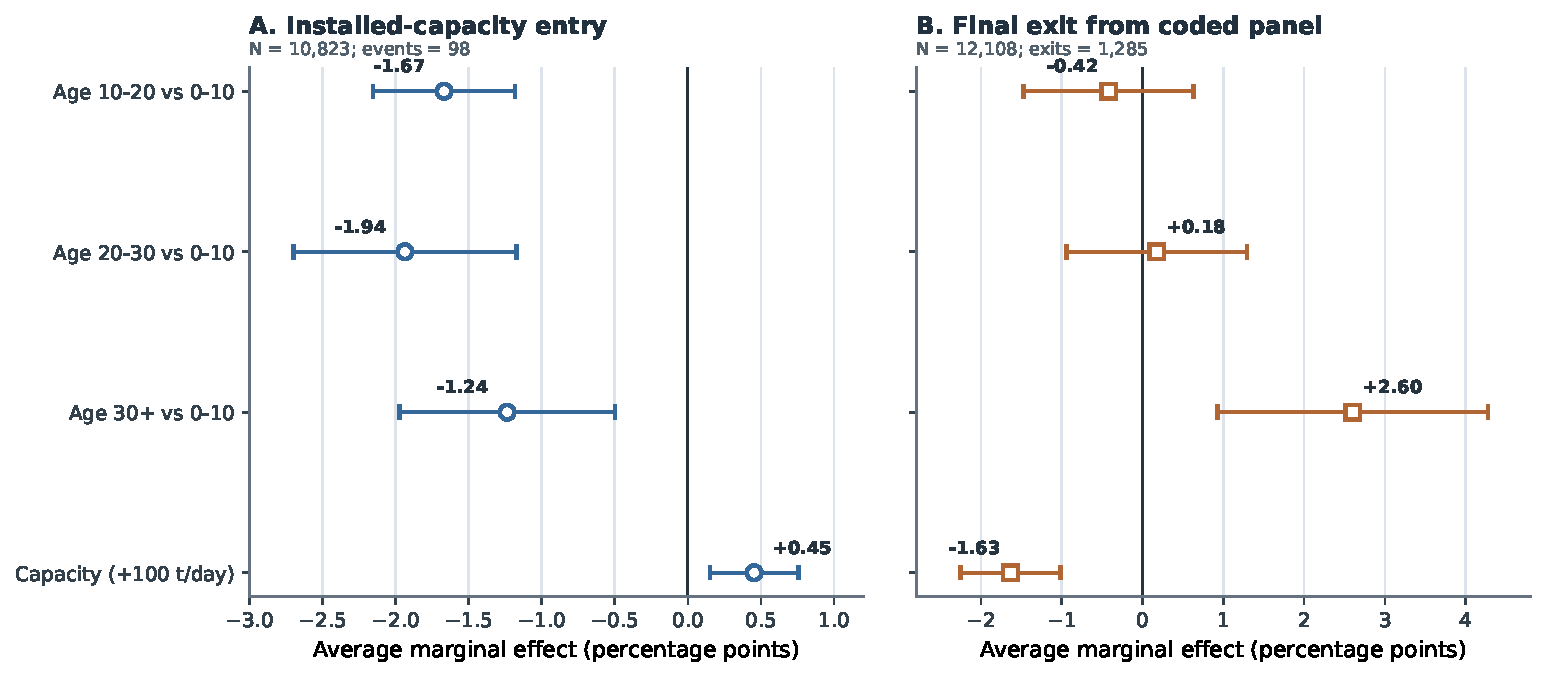
\includegraphics[width=0.90\textwidth]{figure2_selective_transition.pdf}
\caption{Average marginal effects and facility-clustered 95\% confidence intervals for first reporting positive installed generation capacity and final coded-panel exit. Panel exit is not verified closure.}
\end{figure}

\begin{table}[t]
\centering
\caption{Lagged hazard results for installed-capacity entry and coded-panel exit}
\small
\begin{tabularx}{\textwidth}{X R{3.2cm} R{3.2cm}}
\toprule
Variable & Capacity-entry AME (pp) & Panel-exit AME (pp) \\
\midrule
Prior-year age 10--20 years (versus 0--10) & -1.67 (0.25) & -0.42 (0.54) \\
Prior-year age 20--30 years (versus 0--10) & -1.94 (0.39) & 0.18 (0.57) \\
Prior-year age 30+ years (versus 0--10) & -1.24 (0.38) & 2.60 (0.85) \\
Prior-year capacity (per 100 t/day) & 0.45 (0.15) & -1.63 (0.32) \\
\midrule
\multicolumn{3}{l}{\textit{Capacity-entry model summary}} \\
Observations & \multicolumn{2}{r}{10,823} \\
Facilities & \multicolumn{2}{r}{1,911} \\
Installed-capacity entry events & \multicolumn{2}{r}{98} \\
Pseudo-R-squared & \multicolumn{2}{r}{0.1829} \\
\bottomrule
\end{tabularx}
\normalsize
\caption*{\footnotesize Note: entries are average marginal effects (AMEs) in percentage points with standard errors in parentheses, from exact one-fiscal-year lagged logit hazards with fiscal-year indicators and facility-clustered standard errors. The capacity-entry column is the main model; 98 events are retained from a descriptive universe of 141. The exit diagnostic uses 12,108 facility-years, 2,022 facilities, and 1,285 final coded-panel exits before FY2024.}
\end{table}

\subsection{Electricity recovery within generation is strongly structured}

Within the canonical regression frame, generators differ persistently from one another. The within-to-total variance ratio of pooled log electricity-recovery intensity is 0.1499, so most observed variation lies between facilities. More directly, 4,368 exact adjacent-year pairs across 915 facilities have a pooled within-year percentile-rank correlation of 0.9325; the median annual correlation is 0.9323, with a range of 0.8848--0.9763. A high-performing facility therefore usually remains high-ranked one year later even though its exact MWh/t can change. The variance ratio falls from 0.1795 in FY2005--FY2009 to 0.0956 in FY2013--FY2024. This is not a Fukushima identification design because FY2010--FY2012 generator rows lack official facility codes. These diagnostics show persistence, not causal isolation of vintage from technology, governance, maintenance, or other durable characteristics.

The coefficient patterns point in the same direction. Electricity recovery intensity is consistently lower at older facilities and higher at larger and more fully utilized ones. The magnitudes differ across models, but the sign pattern is stable. The emphasis is therefore on structured conditional association rather than on a causal estimate of what would happen if a plant's age, capacity, or utilization were changed by policy. This is consistent with earlier facility-level work showing that energy recovery performance is uneven across operating incinerators and that plant scale and operational intensity matter for output performance (Chen et al., 2012; Yeh, 2020; Grosso et al., 2010). What this paper adds is the linked comparison to the non-generating segment: the same fleet that shows selective entry at one margin also shows a stable hierarchy among mature generators at the other. The supplemental within-between sensitivity preserves the same directional pattern in the cross-facility component: between-facility age is negative, while between-facility capacity and utilization are positive.

\begin{figure}[t]
\centering
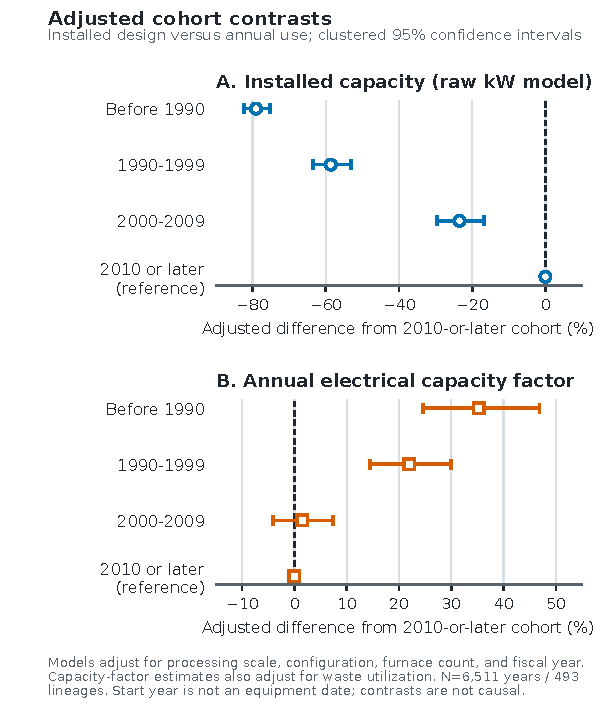
\includegraphics[width=0.975\textwidth]{figure3_efficiency_structure.pdf}
\caption{Mean bounded gross electricity generation per tonne by facility-age group with facility-clustered 95\% confidence intervals, and adjacent-year within-year percentile-rank correlations.}
\end{figure}

The electricity-recovery margin therefore looks structured rather than static. Facilities vary through utilization and operating conditions, but age and scale hierarchies remain strong in the observed data. This is where the paper diverges from a simple engineering-upgrade narrative. Recent large-scale Chinese studies show that substantial gains can still be unlocked through technology upgrades, pollutant control, waste classification, and load-rate improvements, but they do so within already-generating systems rather than at the point of first entry (Liu et al., 2025; Han et al., 2025). The present results are consistent with persistent generator hierarchy rather than natural convergence after entry.

This is why the intensive margin cannot be inferred from the entry margin alone. A facility can report installed capacity and produce electricity while still occupying a different relative performance position from its peers. The data do not establish how much a specific operational intervention could close those gaps. They show structured and highly persistent performance rather than a simple continuation of capacity entry.

For interpretation, this matters as much as the entry result. If the paper only documented selective entry, a reader could infer that the main task was simply to push more facilities into generation. If it only documented generator hierarchy, a reader could infer that non-generators were lagging versions of the same problem. The linked result makes both shortcuts inadequate.

\begin{table}[t]
\centering
\caption{Core electricity-recovery specifications in the canonical generator frame}
\scriptsize
\setlength{\tabcolsep}{5pt}
\resizebox{\textwidth}{!}{%
\begin{tabular}{lrrrr}
\toprule
Variable & Model 1 Pooled OLS & Model 2 Year indicators & Model 3 RE & Model 4 Year indicators + RE \\
\midrule
Facility age (years) & -0.0277*** & -0.0348*** & -0.0136*** & -0.0332*** \\
 & (0.0022) & (0.0023) & (0.0025) & (0.0021) \\
Capacity (100 t/day) & 0.0853*** & 0.1051*** & 0.0340*** & 0.0522*** \\
 & (0.0083) & (0.0087) & (0.0084) & (0.0096) \\
Capacity utilization & 0.7462*** & 0.7760*** & 0.5801*** & 0.5434*** \\
 & (0.1417) & (0.1351) & (0.1086) & (0.0939) \\
Heating value (MJ/kg) & 0.0008 & 0.0033 & -0.0001 & 0.0012 \\
 & (0.0023) & (0.0021) & (0.0013) & (0.0010) \\
Observations & 5,683 & 5,683 & 5,683 & 5,683 \\
Facilities & 1,016 & 1,016 & 1,016 & 1,016 \\
R-squared & 0.2453 & 0.3699 & 0.1148 & 0.3074 \\
\bottomrule
\end{tabular}}
\normalsize
\caption*{\footnotesize Note: OLS means ordinary least squares, RE means random effects, and MJ/kg means megajoules per kilogram. Year indicators are fiscal-year dummy variables, not facility fixed effects. Standard errors are clustered by facility and reported in parentheses. Three asterisks denote $p<0.01$. Coefficients are conditional associations rather than causal structural parameters.}
\end{table}

\subsection{Why the two results belong together}

Read together, the two margins change the modernization story. Some facilities still need to enter energy recovery, while others already generate but remain far apart in performance. The adoption results show selective entry before generator performance is considered. The electricity-recovery results show that large gaps inside the generating segment are not easily erased through within-facility movement alone. A one-average-fleet model would flatten those margins into a single modernization narrative and understate both the selectivity of entry and the persistence of cross-facility performance differences. The point is not that the two samples form one strict causal chain. It is that they locate different observable constraints within the same fleet: who gets into generation, and how far operating generators can move once they are already there.

The post-entry bridge makes the connection observable without claiming a causal sequence. Of 141 installed-capacity entrants, 137 appear in the canonical operating-generator frame within three years. At first appearance, mean gross generation is 0.328 MWh/t, nearly identical to the 0.328 MWh/t same-year mean among incumbent generators. Only three entrants reverse the capacity flag in an observed next year. Capacity entry is therefore usually followed by measurable operation, but it does not guarantee a superior position within the persistent hierarchy. On the other side, panel exit is a competing administrative path for non-entrants. Because exit is not verified closure, the data reveal observed paths rather than a complete physical fate model.

\section{Discussion}

The paper's main interpretive claim is methodological: installed-capacity entry and performance after entry are different problems. Modeling them separately prevents the no-capacity segment and mature generators from being collapsed into one muted fleet mean. That separation reveals selective entry, competing panel exit, and persistent generator hierarchy.

The substantive interpretation is correspondingly two-part. On the entry margin, positive installed capacity is concentrated among younger and larger facilities, while older non-entrants are more likely to disappear from the coded panel. On the electricity-recovery margin, age, scale, and utilization matter within the canonical frame, and adjacent-year ranks are highly persistent. The post-entry bridge supports continuity between the samples without making entry a causal determinant of performance.

This makes the paper useful as a planning diagnostic rather than as an intervention ranking. The practical value is triage: deciding which part of the fleet needs an entry-side asset question and which part needs a generator-side performance question. Table 4 translates the empirical patterns into defensible planning questions while keeping the claim boundaries explicit. In practical terms, the design gives planners a screening sequence: first decide whether a facility is an entry-side asset problem or an already-generating performance problem, then decide which more detailed engineering, governance, or capital-history review is worth pursuing.

\begin{table}[htbp]
\centering
\caption{Planning diagnostic implied by the two-margin evidence}
\small
\begin{tabularx}{\textwidth}{L{3.25cm} >{\raggedright\arraybackslash}X >{\raggedright\arraybackslash}X}
\toprule
Empirical pattern & Planning use & Boundary condition \\
\midrule
Younger/larger entry & Screen non-generators by age, scale, and replacement timing before assuming a simple retrofit path & Older or smaller plants are not proven unable to upgrade \\
Mixed event pathways & Check asset histories before treating adoption as one retrofit mechanism & The audit does not distinguish replacement, refurbishment, and reporting change with certainty \\
Older/smaller panel exit & Verify closure, recoding, consolidation, or reporting status before interpreting continued non-entry & Administrative disappearance is not verified closure \\
Structured generator performance & Compare generators with similar age, scale, and utilization before judging improvement room & Coefficients are conditional associations, not causal effects \\
Persistent adjacent-year ranks & Separate incremental operating improvements from capital-renewal or consolidation decisions & Persistence does not prove plant-specific gains are impossible \\
\bottomrule
\end{tabularx}
\normalsize
\end{table}

The interpretation has clear limits. The pathway audit does not prove a unique mechanism, and the regressions do not provide causal estimates for all Japanese generators. Installed capacity may not describe usable capacity, gross output does not equal net export, useful heat is not measured, and panel exit is not verified closure. Reporting compression, unobserved retrofit histories, governance differences, and institutional constraints remain possible. The defended claim is therefore selective observed entry and persistent generator hierarchy, not a causal intervention ranking.

The results do not identify the best intervention for any individual municipality. They indicate that planning assessments should first distinguish facilities outside electricity recovery from operating generators, because the observable constraints differ across those two groups. For the non-generating energy-recovery segment, especially older non-generators and small plants, the evidence supports diagnostic screening for whether renewal, consolidation, or continued non-generation is plausible. For the already-generating segment, the evidence supports a different diagnostic question: whether an existing generator has realistic room for operational or capital improvement within its observed age, scale, and utilization context.

That distinction is administrative as well as technical. Japanese waste systems are organized through municipalities whose planning boundaries do not always align with efficient waste sheds, and intermunicipal reorganization has its own political costs and institutional legacies (Rausch, 2006; Sakai et al., 2008). In that setting, collapsing non-generators and generators into one average segment risks hiding the difference between entry-side asset decisions, which are lumpy and governance-heavy, and generator performance assessment, which is more incremental and operational.

This distinction also explains why the result is more than a restatement that newer or larger facilities perform better. If both margins were one common process, a single fleet-average modernization story would be adequate. The evidence instead points to two diagnostic starting points: observed entry into generation is selective before performance is measured, and performance remains structured after entry has already occurred.

The analytical split may transfer beyond Japan, but the coefficients do not. It is most relevant where administrative data contain both facilities without energy-recovery equipment and repeated output records for generators. Replication elsewhere requires locally valid identifiers, capacity definitions, closure histories, electricity-use boundaries, and governance variables. Where nearly all plants generate or net heat and electricity exports are measured jointly, the relevant margins would differ.

The broader policy context points in the same direction. Comparative waste policy studies and European framework discussions both treat waste-to-energy as valuable only when embedded inside a wider hierarchy that preserves prevention, reuse, and recycling priorities (Sakai et al., 2011; European Commission, 2017). The empirical split helps explain why those hierarchies matter. A municipal system can have real energy-recovery gains available at the non-generating margin while still facing a different, narrower set of decisions inside the already-generating segment.

For climate interpretation, the relevant question is not simply whether a plant generates, but what kind of generator it is and how much improvement remains inside that segment. Waste-to-energy performance is judged against both an internal engineering standard and the emissions profile of the broader energy system, including the avoided-emissions logic built into carbon accounting (Astrup et al., 2009; M\"{u}nster \& Meibom, 2010). In Japan's current decarbonization setting, where national inventories and scenario work track sectoral emissions and energy mix changes, the two-part design is useful because it keeps those questions separate (Greenhouse Gas Inventory Office of Japan \& Ministry of the Environment Japan, 2024; Yamada et al., 2023).

That separation is also what makes the paper more understandable for a planning audience. Municipal systems rarely choose among abstract technological ideals. They decide whether to renew an aging non-generator, coordinate waste routing toward a larger plant, maintain an existing generator, or invest in an upgrade for a plant that already produces electricity. Those are related decisions, but they are not interchangeable. Keeping the extensive and intensive margins separate helps planners locate the bottleneck without relying on one blended fleet mean.

\section{Conclusion}

In the observed facility panel, Japan's electricity-recovery modernization does not appear as one smooth fleet-wide process. First reporting of positive installed generation capacity is selective, while final coded-panel exit is a competing observed outcome. Within the canonical generator frame, electricity recovery remains stratified by age, scale, and utilization, with high adjacent-year rank persistence. Most capacity entrants soon report positive output, but entry does not imply superior performance. The paper does not identify one unique pathway or intervention hierarchy; it shows why fleet studies should separate capacity entry, administrative attrition, and conditional generator performance.

\section*{Acknowledgements}

The author thanks Prof. Han Ji for supervision and critical feedback during the development of the underlying thesis project from which this paper is derived.

\section*{Funding}

This research did not receive any specific grant from funding agencies in the public, commercial, or not-for-profit sectors.

\section*{Contributor Roles Taxonomy (CRediT) Authorship Contribution Statement}

Pann Phetra: Conceptualization, Data curation, Formal analysis, Investigation, Methodology, Visualization, Writing -- original draft, Writing -- review \& editing.

\section*{Declaration of Competing Interest}

The author declares no known competing financial interests or personal relationships that could have appeared to influence the work reported in this paper.

\section*{Ethical Approval}

This study uses publicly released administrative facility data and does not involve human participants, animal subjects, or private personal data.

\section*{Data Availability}

The facility-level source data are derived from the publicly released Ministry of the Environment Japan General Waste Treatment Survey. Subject to source-file redistribution conditions, the author will deposit the analysis code, machine-readable result manifests, derived tables, figure-generation scripts, and manuscript figures in a versioned repository associated with the submitted paper. Raw workbooks can be obtained from the Ministry and e-Stat portals.

\section*{Declaration of Generative AI and AI-Assisted Technologies in the Manuscript Preparation Process}

During preparation, the author used OpenAI Codex and Anthropic Claude for language revision, manuscript organization, and assistance with code development and review. The author executed the analyses, inspected source data and generated outputs, independently checked reported results, reviewed and edited all AI-assisted material, and takes full responsibility for the content. These tools were not used as authors and did not replace author judgment or accountability.

\section*{References}

\begingroup
\footnotesize
\setlength{\parskip}{0.35em}
\hangindent=1.5em \hangafter=1
\hangindent=1.5em \hangafter=1
Allison, P. D. (1982). Discrete-time methods for the analysis of event histories. \emph{Sociological Methodology, 13}, 61--98. \url{https://doi.org/10.2307/270718}

\hangindent=1.5em \hangafter=1
Astrup, T., M\o ller, J., \& Fruergaard, T. (2009). Incineration and co-combustion of waste: Accounting of greenhouse gases and global warming contributions. \emph{Waste Management \& Research, 27}(8), 789--799. \url{https://doi.org/10.1177/0734242X09343774}

\hangindent=1.5em \hangafter=1
Astrup, T. F., Tonini, D., Turconi, R., \& Boldrin, A. (2015). Life cycle assessment of thermal waste-to-energy technologies: Review and recommendations. \emph{Waste Management, 37}, 104--115. \url{https://doi.org/10.1016/j.wasman.2014.06.011}

\hangindent=1.5em \hangafter=1
Beck, N., Katz, J. N., \& Tucker, R. (1998). Taking time seriously: Time-series-cross-section analysis with a binary dependent variable. \emph{American Journal of Political Science, 42}(4), 1260--1288. \url{https://doi.org/10.2307/2991857}

\hangindent=1.5em \hangafter=1
Brunner, P. H., \& Rechberger, H. (2015). Waste to energy -- key element for sustainable waste management. \emph{Waste Management, 37}, 3--12. \url{https://doi.org/10.1016/j.wasman.2014.02.003}

\hangindent=1.5em \hangafter=1
Cui, J., Cui, Y., Li, J., Gao, X., Wei, W., Chen, Y., Ma, W., Zhu, N., Geng, Y., Zhao, Y., \& Lou, Z. (2026). Efficiency hierarchy and optimization of waste incineration in China to balance disposal and energy supply. \emph{Nature Communications, 17}(1), Article 3069. \url{https://doi.org/10.1038/s41467-026-69897-w}

\hangindent=1.5em \hangafter=1
Chen, P.-C., Chang, C.-C., Yu, M.-M., \& Hsu, S.-H. (2012). Performance measurement for incineration plants using multi-activity network data envelopment analysis: The case of Taiwan. \emph{Journal of Environmental Management, 93}(1), 95--103. \url{https://doi.org/10.1016/j.jenvman.2011.08.011}

\hangindent=1.5em \hangafter=1
e-Stat. (n.d.). \emph{Nation Survey on the State of Discharge and Treatment of Municipal Solid Waste} (Statistics code 00650101). Portal Site of Official Statistics of Japan. \url{https://www.e-stat.go.jp/en/statistics/00650101} (accessed 10 July 2026).

\hangindent=1.5em \hangafter=1
European Commission. (2017). \emph{The role of waste-to-energy in the circular economy} (COM(2017) 34 final). European Commission. \url{https://eur-lex.europa.eu/legal-content/EN/TXT/?uri=CELEX:52017DC0034}

\hangindent=1.5em \hangafter=1
Geels, F. W. (2004). From sectoral systems of innovation to socio-technical systems: Insights about dynamics and change from sociology and institutional theory. \emph{Research Policy, 33}(6--7), 897--920. \url{https://doi.org/10.1016/j.respol.2004.01.015}

\hangindent=1.5em \hangafter=1
Greenhouse Gas Inventory Office of Japan \& Ministry of the Environment Japan. (2024). \emph{National greenhouse gas inventory report of Japan 2024}. Center for Global Environmental Research, National Institute for Environmental Studies. \url{https://cger.nies.go.jp/publications/report/i170/en/}

\hangindent=1.5em \hangafter=1
Grosso, M., Motta, A., \& Rigamonti, L. (2010). Efficiency of energy recovery from waste incineration, in the light of the new Waste Framework Directive. \emph{Waste Management, 30}(7), 1238--1243. \url{https://doi.org/10.1016/j.wasman.2010.02.036}

\hangindent=1.5em \hangafter=1
Han, Q.-l., Liu, H.-q., Gong, Y.-y., Tao, J.-y., Sun, Y.-n., Wei, G.-x., Zhu, Y.-w., \& Chen, G.-y. (2025). Strengthening pollutant control and resource recovery can enhance sustainable waste incineration in China. \emph{Communications Earth \& Environment, 6}, Article 863. \url{https://doi.org/10.1038/s43247-025-02859-0}

\hangindent=1.5em \hangafter=1
Liu, B., Wang, P., Zhou, J., Guo, Y., Ma, S., Chen, W.-Q., Li, J., \& Chang, V. W.-C. (2025). Refocusing on effectiveness over expansion in urban waste-energy-carbon development in China. \emph{Nature Energy, 10}, 215--225. \url{https://doi.org/10.1038/s41560-024-01683-8}

\hangindent=1.5em \hangafter=1
Ministry of the Environment Japan. (2026). \emph{General Waste Treatment Survey results: FY2024 municipal solid waste treatment survey}. Environmental Management Bureau, Ministry of the Environment Japan. \url{https://www.env.go.jp/recycle/waste_tech/ippan/} (accessed 10 July 2026).

\hangindent=1.5em \hangafter=1
M\"{u}nster, M., \& Meibom, P. (2010). Long-term affected energy production of waste to energy technologies identified by use of energy system analysis. \emph{Waste Management, 30}(12), 2510--2519. \url{https://doi.org/10.1016/j.wasman.2010.04.015}

\hangindent=1.5em \hangafter=1
Rausch, A. (2006). The Heisei Dai Gappei: A case study for understanding the municipal mergers of the Heisei era. \emph{Japan Forum, 18}(1), 133--156. \url{https://doi.org/10.1080/09555800500498558}

\hangindent=1.5em \hangafter=1
Sakai, S., Ikematsu, T., Hirai, Y., \& Yoshida, H. (2008). Unit-charging programs for municipal solid waste in Japan. \emph{Waste Management, 28}(12), 2815--2825. \url{https://doi.org/10.1016/j.wasman.2008.07.010}

\hangindent=1.5em \hangafter=1
Sakai, S., Yoshida, H., Hirai, Y., Asari, M., Takigami, H., Takahashi, S., Tomoda, K., Peeler, M. V., Wejchert, J., Schmid-Unterseh, T., Douvan, A. R., Hathaway, R., Hylander, L. D., Fischer, C., Oh, G. J., Jinhui, L., \& Chi, N. K. (2011). International comparative study of 3R and waste management policy developments. \emph{Journal of Material Cycles and Waste Management, 13}(2), 86--102. \url{https://doi.org/10.1007/s10163-011-0009-x}

\hangindent=1.5em \hangafter=1
Seto, K. C., Davis, S. J., Mitchell, R. B., Stokes, E. C., Unruh, G., \& Urge-Vorsatz, D. (2016). Carbon lock-in: Types, causes, and policy implications. \emph{Annual Review of Environment and Resources, 41}(1), 425--452. \url{https://doi.org/10.1146/annurev-environ-110615-085934}

\hangindent=1.5em \hangafter=1
Sun, L., Fujii, M., Tasaki, T., Dong, H., \& Ohnishi, S. (2018). Improving waste to energy rate by promoting an integrated municipal solid-waste management system. \emph{Resources, Conservation and Recycling, 136}, 289--296. \url{https://doi.org/10.1016/j.resconrec.2018.05.005}

\hangindent=1.5em \hangafter=1
Tabata, T., \& Tsai, P. (2016). Heat supply from municipal solid waste incineration plants in Japan: Current situation and future challenges. \emph{Waste Management \& Research, 34}(4), 345--351. \url{https://doi.org/10.1177/0734242X15617009}

\hangindent=1.5em \hangafter=1
Uno, S. (2015). Trends in Waste-to-Energy Technologies for High Efficiency Power Generation. \emph{Material Cycles and Waste Management Research, 26}(2), 114--119. \url{https://doi.org/10.3985/mcwmr.26.114}

\hangindent=1.5em \hangafter=1
Unruh, G. C. (2000). Understanding carbon lock-in. \emph{Energy Policy, 28}(12), 817--830. \url{https://doi.org/10.1016/S0301-4215(00)00070-7}

\hangindent=1.5em \hangafter=1
Wooldridge, J. M. (2010). \emph{Econometric analysis of cross section and panel data} (2nd ed.). MIT Press.

\hangindent=1.5em \hangafter=1
Yamada, K., Ii, R., Yamamoto, M., Ueda, H., \& Sakai, S. (2023). Japan's greenhouse gas reduction scenarios toward net zero by 2050 in the material cycles and waste management sector. \emph{Journal of Material Cycles and Waste Management, 25}(4), 1807--1823. \url{https://doi.org/10.1007/s10163-023-01650-7}

\hangindent=1.5em \hangafter=1
Yeh, L.-T. (2020). Analysis of the dynamic electricity revenue inefficiencies of Taiwan's municipal solid waste incineration plants using data envelopment analysis. \emph{Waste Management, 107}, 28--35. \url{https://doi.org/10.1016/j.wasman.2020.03.040}

\endgroup

\end{document}
